\chapter{Métricas de Software}
\label{chap:metricas}

Esse capítulo será responsável pela explicação teórica a respeito do que são métricas de código e como elas foram utilizadas no desenvolvimento da solução que esse trabalho busca analisar. A explicação teórica envolve desde o entendimento do processo de medição descrito pela \citeonline{ISO:15939} até a explicação sobre intervalos qualitativos para valores de cada métrica de código fonte propostos por \citeonline{Meirelles2013}. Por fim, serão apresentados os cenários de limpeza de código utilizados nesse trabalho para monitoramento da qualidade do código fonte.

\section{Processo de Medição}

A \citeonline{ISO:15939} define medição como a união de operações cujo objetivo é atribuir um valor a uma métrica. Graças ao processo de medição é possível entender e controlar o que está acontecendo durante o processo de desenvolvimento e manutenção de um sistema \citeonline{Fenton98}. Ainda segundo a \citeonline{ISO:15939}, o processo de medição é a chave primária para a gerência de um software e suas atividades no seu ciclo de vida, além disso, um processo de melhoria contínua requer mudanças evolutivas e mudanças evolutivas requerem um processo de medição.
	Complementando o conceito levantado anteriormente, é possível afirmar de acordo com a \citeonline{ISO:9126} que a medição é a utilização de uma métrica para  atribuir um valor, que pode ser um número ou uma categoria, obtido a partir de uma escala a um atributo de uma entidade.
	A escala, citada anteriormente, pode ser definida como um conjunto de categorias para as quais os atributos estão mapeados, de modo que um atributo de medição está associado a uma escala \citeonline{ISO:15939}. Essas escalas podem ser divididas em:	

	\begin{easylist}[itemize]

& \textbf{Nominal:} São empregadas expressões semânticas para representar objetos para fins de identificação \cite{pandian_software_2004}. Na interpretação dos valores de cada atributo, a ordem não possui significado \cite{Meirelles2013}.

& \textbf{Ordinal:} Os valores podem ser comparados em ordem, é possível agrupar valores em categorias também podem ser ordenadas. Porém esta escala não oferece informações sobre a magnitude da diferença entre os elementos \cite{metricsandmodels}.


& \textbf{Intervalo:} A ordem dos resultados é importante, assim como o tamanho dos intervalos que separam os pontos, mas a proporções não são necessariamente válidas \cite{Meirelles2013}. Operações matemáticas como adição e subtração podem ser aplicadas a este tipo de intervalo \cite{metricsandmodels}.

& \textbf{Racional:} Possui a mesma definição da escala de intervalo, a diferença está no fato da proporção ser preservada \cite{Meirelles2013}. Ou seja, é possível definir um unidade zero para um tamanho de unidade previamente estabelecido pela escala \cite{metricsandmodels}.


\end{easylist}
	
	A \citeonline{ISO:15939} divide o processo de medição em dois métodos diferentes, que se distinguem pela natureza do que é quantificado:
	
	\begin{easylist}[itemize]

	& \textbf{Subjetiva:} Quantificação envolvendo julgamento de um humano
	& \textbf{Objetiva:} Quantificação baseada em regras numéricas. Essas regras podem ser implementadas por um humano.

	\end{easylist}


%---------------------------------------------------------------------------------------------------------------------%

\section{Definição das Métricas de Software}

\citeonline{Fenton98}, mostraram que o termo métricas de software abrange muitas atividades, as quais estão envolvidas em um certo grau de medição de um software, como por exemplo estimativa de custo, estimativa de esforço e capacidade de reaproveitamento de elementos do software. Nesse contexto \citeonline{ISO:9126} categoriza as seguintes métricas de acordo com os diferentes tipos de medição:

\begin{easylist}[itemize]

 & \textbf{Métricas internas:} Aplicadas em um produto de software não executável, como código fonte. Oferecem aos usuários, desenvolvedores ou avaliadores o benefício de poder avaliar a qualidade do produto antes que ele seja executável.
& \textbf{Métricas externas:} Aplicadas a um produto de software executável, medindo o comportamento do sistema do qual o software é uma parte através de teste, operação ou mesmo obervação. Oferecem aos usuários, desenvolvedores ou avaliadores o benefício de poder avaliar a qualidade do produto durante seu processo de teste ou operação.
& \textbf{Métricas de qualidade em uso:} Aplicadas para medir o quanto um produto atende as necessidades de um usuário para que sejam atingidas metas especificadas como eficácia, produtividade, segurança e satisfação.

\end{easylist}

A Figura \ref{fig:modelodequalidade} reflete como as métricas influenciam nos contextos em que elas estão envolvidas, seja em relação ao software propriamente dito (tanto internamente quanto externamente) ou ao efeito produzido pelo uso de software:

	
\begin{figure}[h!]
\centering
\includegraphics[keepaspectratio=false,scale=0.90]{figuras/figuras_matheus/tipos_medidas_INGLES.eps}
\caption{Modelo de Qualidade do Produto adaptado da 
\citeonline{ISO25023}}
\label{fig:modelodequalidade}
\end{figure}
\FloatBarrier

%---------------------------------------------------------------------------------------------------------------------%

\section{Métricas de Código Fonte}

Serão utilizadas nesse trabalho de conclusão de curso métricas de código fonte, que segundo \citeonline{Meirelles2013} são métricas do tipo objetiva calculadas a partir da análise estática do código fonte de um software. As métricas de código fonte serão divididas em duas categorias, seguindo a categorização adotada por \citeonline{rego_monitoramento_2014}: Métricas de tamanho e complexidade e métricas de orientação a objetos.

%--------------------------------------------
\subsection{Métricas de Tamanho e Complexidade}

O tamanho do código-fonte de um sistema foi um dos primeiros conceitos mensuráveis de software, uma vez que softwares podiam ocupar espaço tanto em forma de cartão perfurado quanto em forma de papel quando o código era impresso. Na programação em Assembler, por exemplo, uma linha física de código era o mesmo que uma instrução, logo, quanto maior o tamanho do código, maior era sua complexidade \cite{metricsandmodels}. A seguir são apresentadas algumas métricas de tamanho e complexidade.

\begin{easylist}[itemize]

	& \textbf{LOC} (\textit{Lines of Code}): Métrica simples em que são contadas as linhas executáveis de um código, desconsiderando linhas em branco e comentários.  \cite{metricsandmodels} 
		
	& \textbf{ACCM} (\textit{Average Cyclomatic Complexity per Method}): Mede a complexidade do programa, podendo ser representada através de um grafo de fluxo de controle. \cite{McCabe76}

	& \textbf{AMLOC} (\textit{Average Method Lines of Code}): Indica a distribuição de código entre os métodos. Quanto maior o valor da métrica, mais pesado é o método. É preferível que haja muitos métodos com pequenas operações do que um método grande e de entendimento complexo. \cite{Meirelles2013}
	
\end{easylist}

\subsection{Métricas de Orientação a Objetos}

O surgimento da programação orientada a objetos representou uma importante mudança na estratégia de desenvolvimento, focalizando a atenção para conceitos mais próximos ao negócio modelado. \cite{phpmysql}  

Métricas de orientação a objetos foram adotadas devido à grande utilização desse paradigma no desenvolvimento de software. Serão adotadas as seguintes métricas já selecionadas por \citeonline{rego_monitoramento_2014}:  

\begin{easylist}
	
	%--------------------------
	& \textbf{ACC} (\textit{Afferent Connections per Class} - Conexões Aferentes por Classe): Mede a conectividade entre as classes. Quanto maior a conectividade entre elas, maior o potencial de impacto que uma alteração pode gerar. \cite{Meirelles2013}
	
	%--------------------------
	& \textbf{ANPM} (\textit{Average Number of Parameters per Method} - Média do Número de Parâmetros por Método): Indica a média de parâmetros que os métodos possuem. Um valor muito alto para quantidade de parâmetros pode indicar que o método está tendo mais de uma responsabilidade. \cite{Basili1987}

	%--------------------------
	& \textbf{CBO} (\textit{Coupling Between Objects} - Acoplamento entre Objetos): Essa é uma métrica que diz respeito a quantas outras classes dependem de uma classe. É a conta das classes às quais uma classe está acoplada. 		Duas classes estão acopladas quando métodos de uma delas utilizam métodos ou variáveis de outra. Altos 			valores dessa métrica aumentam a complexidade e diminuem a manutenibilidade.  \cite{softwaremeasurementandestimation}. Segundo \citeonline{pressman_engenharia_2010} é provavél que a reusabilidade de uma classe diminua à medida que o CBO aumenta, pois valores altos complicam as modificações e os testes.
  		 
	%-----------------------------
	& \textbf{DIT} (\textit{Depth of Inheritance Tree} - Profundidade da 
	Árvore de Herança): Responsável por medir quantas camadas de herança compõem uma determinada hierarquia 		de classes \cite{softwaremeasurementandestimation}. Quanto mais profunda for a árvore, maior será o número de classes envolvidas \cite{Chidamber-1994}, consequentemente haverá um número maior de métodos e atributos herdados, aumentando assim a complexidade da classe \citeonline{Meirelles2013}.

	%--------------------------
	& \textbf{LCOM4} (\textit{Lack of Cohesion in Methods} - Falta de Coesão
	entre Métodos):Falta de Coesão entre Métodos): Proposta inicialmente por \citeonline{Chidamber-1994}, LCOM calcula o número de métodos que têm acesso a um ou mais atributos de uma dada classe \cite{pressman_engenharia_2010}. Por ter recebido diversas críticas, várias alternativas foram criadas. \citeonline{LCOM4} definiu uma revisão desta métrica e assim elaborou uma outra versão conhecida como LCOM4. Para calcular LCOM4 de um módulo, é necessário construir um gráfico não-orientado em que os nós são os métodos e atribuos de uma classe. Para cada método, deve haver uma areste entre ele e um outro método ou variável que ele usa. O valor da LCOM4 é o número de componentes fracamente conectados nesse gráfico \cite{Meirelles2013}.

	%--------------------------
	& \textbf{NOC} (\textit{Number of Children} - Número de Filhos): É o número de sucessores imediatos (portanto filhos), de uma classe. Segundo \citeonline{softwaremeasurementandestimation}, altos valores indicam que a abstração da super classe foi diluída e uma reorganização da arquitetura deve ser considerada. \citeonline{pressman_engenharia_2010} justifica esse fato afirmando que à medida que o número de filhos cresce, alguns deles não são necessariamente membros adequados da super classe.
	
	%-----------------------------
	& \textbf{NOM} (\textit{Number of Methods} - Número de Métodos): Indica a quantidade de métodos de uma classe, medindo seu tamanho. Classes com muitos métodos são mais difíceis de serem reutilizadas pois são propensas a serem menos coesas. \cite{Meirelles2013}  

	%-----------------------------
	& \textbf{NPA} (\textit{Number of Public Attributes} - Número de Atributos Públicos): Mede o encapsulamento de uma classe, através da medição dos atributos públicos. O número ideal para essa métrica é zero \cite{Meirelles2013}

	%-----------------------------
	& \textbf{RFC} (\textit{Response For a Class} - Respostas para uma Classe): \citeonline{metricsandmodels} define essa métrica como o número de métodos que podem ser executados em respostas a uma mensagem recebida por um objeto da classe.

\end{easylist}	

%---------------------------------------------------------------------------------------------------------------------%

\section{Configurações de Qualidade para Métricas de Código Fonte} 

Em sua tese de doutorado, \citeonline{Meirelles2013} buscou responder as seguintes questões de pesquisa:
\begin{easylist}[itemize]

	& \textbf{QP1 -} Métricas de código-fonte podem influir na atratividade de projetos de software livre? 
	& \textbf{QP1 -} Quais métricas devem ser controladas ao longo do tempo?		
	& \textbf{QP3 -} As métricas de código-fonte melhoram com o amadurecimento do projeto?	
	
\end{easylist}

Para responder essas questões, sua pesquisa concentrou-se em alguns objetivos tecnológicos e científicos, fazendo uso da técnica estatística descritiva percentil para identificação das distribuições dos valores de métricas em 38 projetos de software livre, observando os valores frequentes dessas métricas de modo a servirem de referência para projetos futuros. 

O percentil são pontos estimativos de uma distribuição de frequência que determinam a porcentagem de elementos que se encontram abaixo deles. Por exemplo, quando se diz que o valor 59,0 da métrica rfc do projeto \textbf{Open JDK8} está no percentil 90, significa dizer que 90\% dos valores identificados para essa métrica estão abaixo de 59,0. 

A tabela \ref{tab:percentil} abaixo pôde ser criada graças ao uso da técnica estatística citada:
	
	\begin{table}[!ht]
	\begin{center}
	
	\input{tabelas/tabelasMatheus/percentis.ltx} 
	\caption{Percentis para métrica RFC em projetos Java extraídos de  
	\citeonline{Meirelles2013}}
	\label{tab:percentil}
	\end{center}
	\end{table}	
	\FloatBarrier	

Através dos resultados obtidos para cada métrica, \citeonline{Meirelles2013} observou que era possível identificar valores frequentes analisando os percentis. Na \ref{tab:percentil}, por exemplo, foram observados no projeto \textbf{Open JDK8} valores de 0 a 9 como muito frequentes, de 10 a 26 como frequente, de 27 a 59 como pouco frequente e acima de 59, que representa apenas 10\% do código-fonte do projeto, como não frequente \cite{Meirelles2013}. A tabela \ref{tab:nomes} foi extraída do trabalho de conclusão de curso de \citeonline{rego_monitoramento_2014} para que fosse criada uma relação entre o intervalo de frequência e o intervalo qualitativo de uma métrica, afim de facilitar sua interpretação:

\begin{table}[!ht]
	\begin{center}
	\input{tabelas/tabelasMatheus/intervalos.ltx}
	\caption{Nome dos Intervalos de Frequência extraídos de \citeonline{rego_monitoramento_2014}}
	\label{tab:nomes}
	\end{center}
	\end{table}
	\FloatBarrier
	
	 
\citeonline{Meirelles2013} destaca na avaliação dos resultados a maneira como o \textbf{Open JDK8} demonstrou um equilíbrio no valor das métricas em relação aos demais projetos Java, de modo que seus valores são frequentemente usados como referência na interpretação dos valores das métricas. Se de um lado o  \textbf{Open JDK8} demonstrou os menores valores percentis, os valores mais altos foram identificados no \textbf{Tomcat}. \citeonline{rego_monitoramento_2014} considerou então os dois cenários para que as referências de valores para as métricas fossem criadas. O resultado dessa análise gerou em seu trabalho a tabela \ref{tab:good-metrics}:

\begin{table}[!ht]
	\begin{center}
	\input{tabelas/tabelasMatheus/metricas.ltx}	
	\caption{Configurações para os Intervalos das Métricas para Java extraídas de \citeonline{rego_monitoramento_2014}}
	\label{tab:good-metrics}
	\end{center}
	\end{table}
	\FloatBarrier
   

%---------------------------------------------------------------------------------------------------------------------%

\section{Cenários de Limpeza} 

Em seu livro \textit{Implementation Patterns}, \citeonline{Beck2007} destaca três valores que um código limpo precisa ter: Comunicabilidade, simplicidade e flexibilidade.
	
\begin{easylist}[itemize]

	& \textbf{Comunicabilidade:} Um código se expressa bem quando alguém que o lê é capaz de compreendê-lo e modificá-lo. \citeonline{Beck2007} destaca que quando foi necessário modificar um código, ele gastou muito mais tempo lendo o que já havia sido feito do que escrevendo sua modificação 
		
	& \textbf{Simplicidade:} Eliminar o excesso de complexidade faz com que aqueles que estejam lendo o código a entendê-lo mais rapidamente. O excesso de complexidade faz com que seja maior a probabilidade de erro e com que seja mais difícil fazer uma manutenção no futuro.Buscar simplicidade é também buscar inovação: \textit{Junit} é muito mais simples que muitas ferramentas de teste que ele substituiu.

	& \textbf{Flexibilidade:} Capacidade de estender a aplicação alterando o mínimo possível a estrutura já criada.
		
\end{easylist}	

Buscando levantar conceitos que fizessem com que um código atendesse os valores citados acima, tornando-se assim um código limpo, \citeonline{Machini2010} levantou em seu trabalho conceitos de limpeza, evidenciando as contribuições e consequências que o uso da técnica pode causar no código. Serão citadas na tabela \ref{tab:conceitos} técnicas levantadas por \citeonline{Machini2010} que ganharam destaque no trabalho de \citeonline{rego_monitoramento_2014}:

 \begin{table}[!ht]
\centering
\input{tabelas/tabelasMatheus/conceitos-limpeza.ltx}
\caption{Conceitos de Limpeza levantados por \citeonline{Machini2010} extraídos de \citeonline{rego_monitoramento_2014}}
\label{tab:conceitos}
\end{table}
\FloatBarrier

Após o levantamento dos conceitos de limpeza, \citeonline{Machini2010} criou um mapeamento os relacionando com métricas de código, definindo cenários de limpeza. O objetivo, como ressaltado pelo autor, não era classificar um código como limpo ou não, mas sim facilitar melhorias de implementação através da aproximação dos valores das métricas com os esperados nos contextos de interpretação.

Aproveitando inicialmente os cenários \textbf{Classe pouco coesa} e \textbf{Interface dos métodos} extraídos de  \citeonline{Machini2010}, \citeonline{rego_monitoramento_2014} elaborou mais alguns cenários de limpeza, utilizando como referência a configuracão do \textbf{Open JDK8}, considerando como valores altos os valores obtidos pelos intervalos  Regular e Ruim para esse sistema. O resultado dessa atividade pode ser visto na tabela \ref{tab:cenarios}:

\begin{sidewaystable}
\begin{table}[H]
\centering
\input{tabelas/tabelasMatheus/cenarios.ltx}
\caption{Cenários de Limpeza extraídos de \citeonline{rego_monitoramento_2014}}
\label{tab:cenarios}
\end{table}
\FloatBarrier
\end{sidewaystable}  

\section{Considerações Finais do Capítulo}  

Esse capítulo apresentou a fundamentação teórica sobre aquilo que é medido e monitorado pela solução proposta. Além de uma definição sobre o que são métricas de código fonte e quais são seus intervalos qualitativos, também foi apresentada nesse capítulo a maneira como elas foram relacionadas a cenários de limpeza. O próximo capítulo será responsável por apresentar a teoria acerca de \textit{Data Warehousing} e como seu uso pode servir no monitoramento das métricas apresentadas nesse capítulo.